\section{方法}
基于上述研究目标,图~\ref{fig:研究方法}给出了研究方法概述,主要将方法定义为三个步骤:

\begin{enumerate}
    \item 语句生成。基于已有的知识图谱生成语句集,包括同时由事实语句与反事实语句构成、且数据量较大的训练集,以及仅包括反事实语句的验证集。
    \item 模型训练。以生成的训练集为输入,对预训练的语言模型进行训练。
    \item 模型验证。以生成的验证集为输入,对训练好的语言模型进行验证,并对输出结果进行评估。
\end{enumerate}

\begin{figure}[htb]
    \centering
    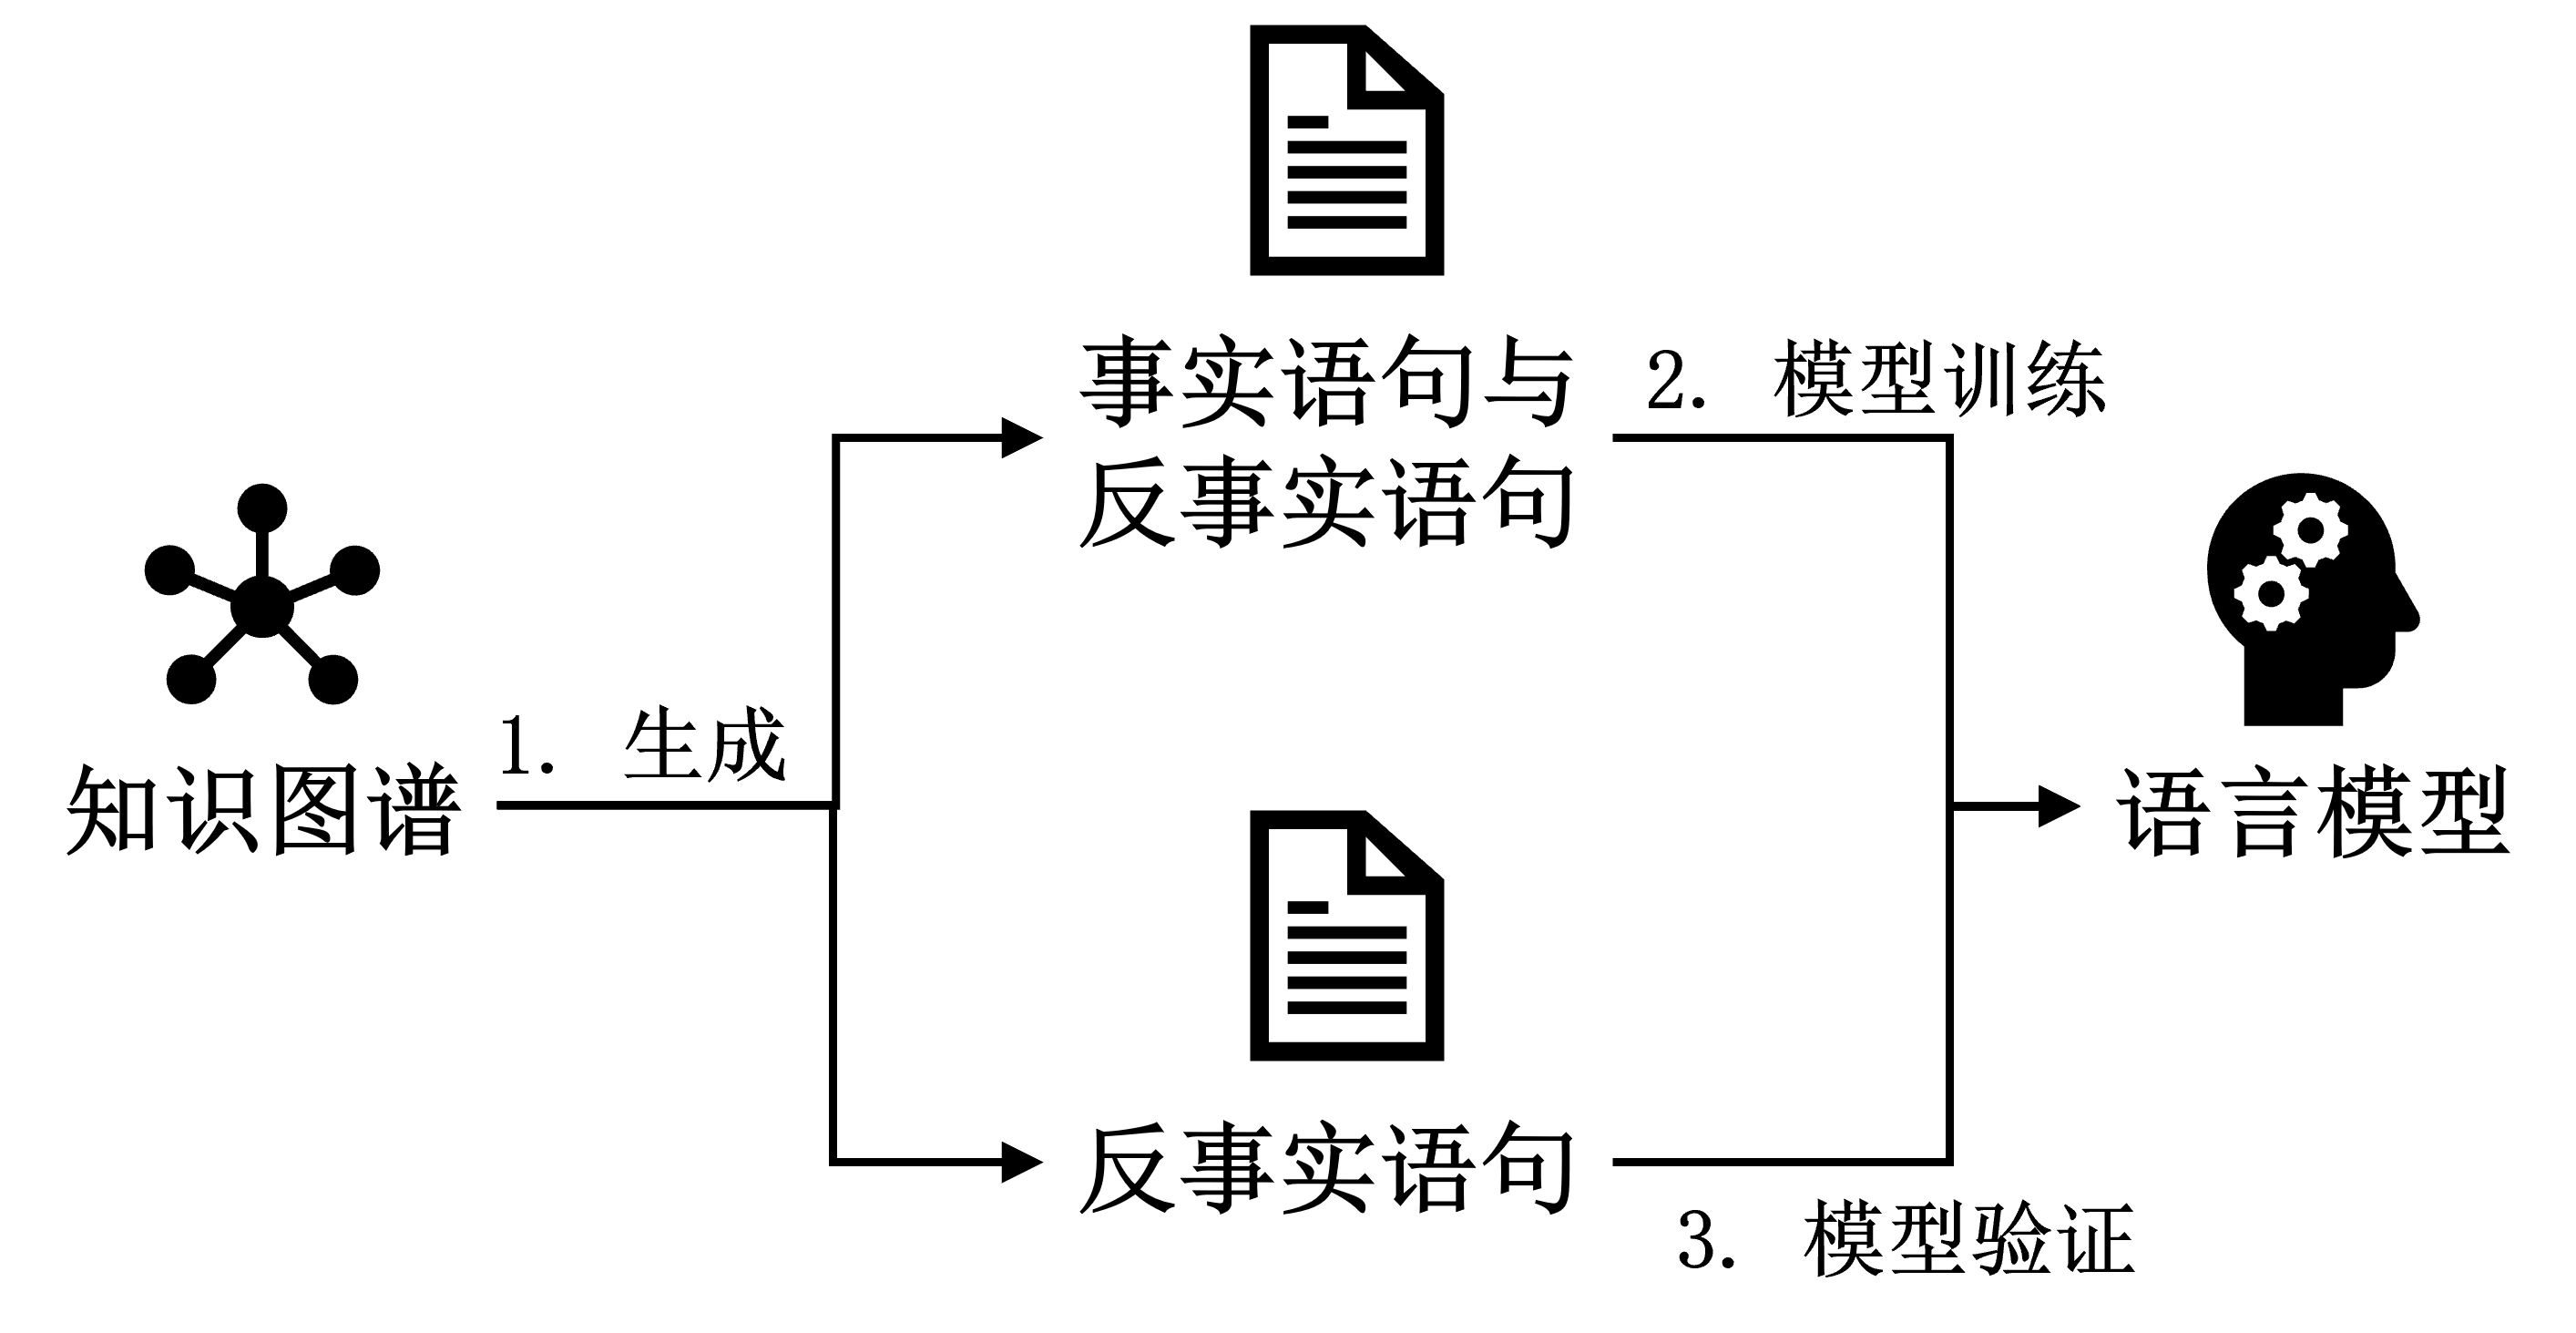
\includegraphics[width=0.5\textwidth]{images/研究方法.png}
    \caption[研究方法]{研究方法}
    \label{fig:研究方法}
\end{figure}

基于上述研究方法与具体步骤,本文将研究问题定义为三个部分,包括知识图谱选择、基于图谱的事实与反事实语句生成、以及语言模型选择。
本节将针对上述定义的三个研究问题进行说明。

\subsection{知识图谱选择}
\subsubsection{数据集选择}
\subsubsection{数据集处理}


\subsection{基于图谱的事实与反事实语句生成}


\subsection{语言模型选择}

